% =====================================================================
%  4. Evaluation
% =====================================================================
\section{Evaluation}
\label{sec:evaluation}

\subsection{Protocol}
\label{sec:protocol}

\paragraph{Metrics.} MAE in MW is the main metric because it has a physical unit. Root mean squared error (RMSE) stresses
large errors. MAPE is reported only for comparison with the literature, and is safe here because load
never approaches zero~\cite{hyndman2021fpp3}. We also report the bias (mean of prediction minus
actual).

\paragraph{Paired comparison.} For models A and B, let $\Delta=\MAE_A-\MAE_B$ (negative means A is
better). Errors of neighbouring hours are strongly autocorrelated, so we resample whole calendar
weeks (2{,}000 block-bootstrap samples~\cite{kunsch1989jackknife}) of the paired differences
$|e_A|-|e_B|$ and take the 95\% percentile interval. With a threshold $\delta$ equal to 2\% of the MAE
of the simpler model of the pair (a heuristic fixed before running the test), the verdict is:
\begin{itemize}
  \item \textbf{clearly better}: the interval excludes 0 and $|\Delta|\ge\delta$;
  \item \textbf{about equal}: the interval lies inside $[-\delta,+\delta]$;
  \item \textbf{undecided}: otherwise.
\end{itemize}
We also count in how many calendar months A beats B, to see whether a gain is broad or comes from a
few weeks.

\paragraph{TSO reference.} The TSO forecast is shown for context only. The TSO has internal data and
weather forecasts, and we do not know exactly when the column was last updated. We therefore do not
claim to beat or lose to it.

\subsection{Validation Results (2017)}
\label{sec:eval-val}

\begin{table}[H]
  \centering
  \small
  \caption{Validation 2017, 8{,}757 hours. Mean load 28{,}858\,MW.}
  \label{tab:val}
  \begin{tabular}{@{}l l r r r r@{}}
    \toprule
    Model & Weather & MAE & RMSE & MAPE (\%) & Bias \\
    \midrule
    B0 seasonal naive & -- & 2{,}627 & 3{,}748 & 9.20 & $-2$ \\
    B1 Ridge & actual & 1{,}840 & 2{,}562 & 6.38 & $-358$ \\
    B1 Ridge & lagged & 1{,}859 & 2{,}594 & 6.44 & $-378$ \\
    M1 LightGBM & actual & 1{,}591 & 2{,}350 & 5.56 & $-316$ \\
    M1 LightGBM & lagged & 1{,}683 & 2{,}438 & 5.89 & $-266$ \\
    \midrule
    TSO (reference) & -- & 314 & 430 & 1.08 & 2 \\
    \bottomrule
  \end{tabular}
\end{table}

\begin{table}[H]
  \centering
  \small
  \caption{Paired comparisons on validation ($\Delta$ in MW, 95\% block-bootstrap interval).}
  \label{tab:val-pairs}
  \begin{tabular}{@{}l l r c c l@{}}
    \toprule
    A & B & $\Delta$ & 95\% interval & Months A better & Verdict \\
    \midrule
    B1 actual & B0 & $-787$ & $[-1045,\,-512]$ & 12/12 & clearly better \\
    B1 lagged & B0 & $-768$ & $[-1036,\,-482]$ & 12/12 & clearly better \\
    B1 actual & B1 lagged & $-19$ & $[-54,\,17]$ & 8/12 & undecided \\
    M1 actual & B1 actual & $-249$ & $[-354,\,-134]$ & 12/12 & clearly better \\
    M1 lagged & B1 lagged & $-175$ & $[-275,\,-71]$ & 10/12 & clearly better \\
    M1 actual & M1 lagged & $-93$ & $[-153,\,-31]$ & 12/12 & clearly better \\
    \bottomrule
  \end{tabular}
\end{table}

On validation, features plus a linear model remove about 30\% of the seasonal-naive error, in every
month. LightGBM removes a further 9--14\% of the Ridge error. Knowing the actual weather helps
LightGBM by 93\,MW but Ridge by only 19\,MW, which is not distinguishable from zero. A possible
reading is that the trees use same-day temperature in a way the degree-day form does not, but this
is not shown yet (\cref{sec:eval-why}).

\paragraph{Resolution.} The half-width of the intervals is 100--110\,MW for M1 versus B1 and
35--60\,MW for actual versus lagged, against thresholds $\delta$ of about 34--37\,MW. Differences
smaller than roughly 100\,MW between models therefore end up ``undecided''. We keep $\delta$
unchanged and state this limit.

\paragraph{Loss versus metric.} Both models train on squared error but are scored by MAE. Removing
the median residual would lower the MAE by 30--50\,MW for both models (e.g.\ 1{,}840 to 1{,}791 for
B1 actual, 1{,}591 to 1{,}554 for M1 actual), so the mismatch affects both models by a similar
amount. This is only a diagnostic; predictions are not corrected.

\begin{table}[H]
  \centering
  \small
  \caption{Validation MAE (MW) by day type. Bold: best of B1/M1 in each weather setting.}
  \label{tab:val-daytype}
  \begin{tabular}{@{}l r r r r r r r@{}}
    \toprule
    Day type & Hours & B0 & B1 actual & M1 actual & B1 lagged & M1 lagged & TSO \\
    \midrule
    Workday & 5{,}950 & 2{,}583 & 1{,}778 & \textbf{1{,}453} & 1{,}802 & \textbf{1{,}553} & 307 \\
    Saturday & 1{,}248 & 2{,}230 & 1{,}606 & \textbf{1{,}541} & 1{,}662 & \textbf{1{,}615} & 316 \\
    Sunday & 1{,}271 & 2{,}974 & 2{,}194 & \textbf{1{,}955} & 2{,}152 & \textbf{2{,}089} & 308 \\
    Holiday & 240 & 4{,}193 & \textbf{2{,}957} & 3{,}451 & \textbf{2{,}984} & 3{,}278 & 466 \\
    Bridge day & 48 & 1{,}439 & \textbf{574} & 1{,}082 & \textbf{634} & 916 & 518 \\
    \bottomrule
  \end{tabular}
\end{table}

LightGBM wins on ordinary days but loses to Ridge on holidays and bridge days
(\cref{tab:val-daytype}). These days are rare (288 hours in the validation year and similarly few in
training), so the trees see few examples. Ridge treats the holiday share as one linear shift per hour,
which generalises from few examples. On the test year this holds only for bridge days
(\cref{sec:eval-why}).

The largest bias is in June 2017 ($-1{,}643$\,MW for B1 actual, $-956$\,MW for M1 actual), the month
of a record heat wave: June load was about 2{,}000\,MW above the June level of the two training
years. With only two training summers, the models had not seen such heat in June. We did not add
features to fix this after seeing the validation year, since that would overfit validation.

\subsection{Test Results (2018)}
\label{sec:eval-test}

The test script ran once on Kaggle (started 2026-11-10 17:16 UTC, after the configuration was frozen
at 16:32 UTC). It verified the SHA-256 (Secure Hash Algorithm) hashes of the frozen parameters and that adding 2018 changed
no feature of any earlier row. One one-hour spike in 2018 (6 May, 12:00) was set to missing by the
cleaning rule; 4 weather hours (clock-change slots) were forward-filled.

\begin{table}[H]
  \centering
  \small
  \caption{Test 2018, 8{,}756 hours (MW). The last column is the change from validation to test.}
  \label{tab:test}
  \begin{tabular}{@{}l l r r r r r@{}}
    \toprule
    Model & Weather & MAE & RMSE & MAPE (\%) & Bias & $\Delta$ vs.\ val. \\
    \midrule
    B0 seasonal naive & -- & 2{,}632 & 3{,}804 & 9.08 & $+13$ & $+5$ \\
    B1 Ridge & actual & 1{,}752 & 2{,}510 & 5.95 & $-402$ & $-88$ \\
    M1 LightGBM & actual & \textbf{1{,}521} & \textbf{2{,}286} & \textbf{5.18} & $-387$ & $-70$ \\
    B1 Ridge & lagged & 1{,}760 & 2{,}525 & 5.96 & $-445$ & $-99$ \\
    M1 LightGBM & lagged & 1{,}592 & 2{,}316 & 5.42 & $-355$ & $-92$ \\
    \midrule
    TSO (reference) & -- & 268 & 367 & 0.92 & $+2$ & $-46$ \\
    \bottomrule
  \end{tabular}
\end{table}

\begin{table}[H]
  \centering
  \small
  \caption{Paired comparisons on the test year ($\Delta$ in MW, 95\% block-bootstrap interval).}
  \label{tab:test-pairs}
  \begin{tabular}{@{}l l r c r c l@{}}
    \toprule
    A & B & $\Delta$ & 95\% interval & \% load & Months A better & Verdict \\
    \midrule
    B1 actual & B0 & $-880$ & $[-1120,\,-649]$ & $-3.0$ & 12/12 & clearly better \\
    B1 lagged & B0 & $-872$ & $[-1124,\,-632]$ & $-3.0$ & 12/12 & clearly better \\
    M1 actual & B1 actual & $-231$ & $[-342,\,-119]$ & $-0.8$ & 10/12 & clearly better \\
    M1 lagged & B1 lagged & $-168$ & $[-277,\,-56]$ & $-0.6$ & 11/12 & clearly better \\
    B1 actual & B1 lagged & $-8$ & $[-39,\,23]$ & $-0.03$ & 4/12 & undecided \\
    M1 actual & M1 lagged & $-71$ & $[-128,\,-11]$ & $-0.25$ & 9/12 & clearly better \\
    \bottomrule
  \end{tabular}
\end{table}

All verdicts are the same as on validation. Every learned model has a \emph{lower} error on the test
year than on validation (70--99\,MW), while the naive floor stays flat. Two reasons are likely: the
final models are trained on three years instead of two (one more summer), and 2018 had no heat wave
as extreme as June 2017. So there is no sign that tuning overfitted the validation year. All learned
models still under-forecast by 350--450\,MW on average (B0 is unbiased).

\begin{figure}[H]
  \centering
  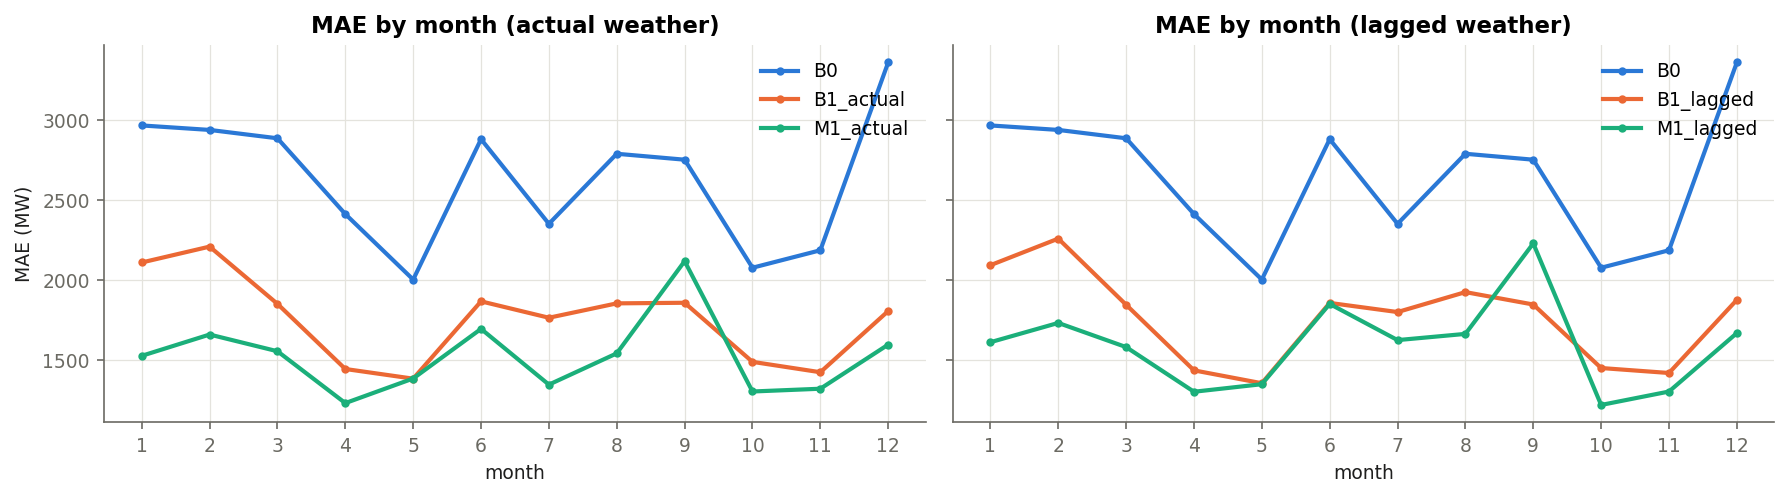
\includegraphics[width=\linewidth]{04_test_mae_by_month.png}
  \caption{Test MAE by month in both weather settings.}
  \label{fig:test-month}
\end{figure}

\paragraph{September 2018.} It is the only month in which LightGBM is clearly worse than Ridge
(\cref{fig:test-month}). The recorded load in early September does not follow the weekday pattern:
Saturday 1 and Sunday 2 September reach 34{,}064 and 34{,}646\,MW (higher than an ordinary
workday), while Thursday 6 and Wednesday 12 September are as low as a Sunday. The TSO forecast column
shows the same pattern within about 1\%, so these values are either real unusual events or a date
misalignment in the source; we cannot tell which. We did not change the test data. In a post-hoc
check (decided after seeing the results, so only supporting evidence), removing September keeps
all verdicts unchanged and widens the LightGBM gain to 275\,MW (actual) and 218\,MW (lagged).

\subsection{Separating Fitting, Features and Structure}
\label{sec:eval-ablation}

\paragraph{Protocol and disclosure.} The variants of \cref{tab:variants} were added \emph{after} the
test results above were known. Their configuration was chosen on validation only, frozen with
SHA-256 hashes and committed, and only then was 2018 loaded a second time, in one run, for these
models only. B0, B1 and M1 were not refitted, so all numbers above are unchanged. A first attempt of
this run stopped at its precondition check before reading any data. On validation the verdicts are
the same as in \cref{tab:ablation}, except that feature engineering for the global Ridge was
undecided in the lagged setting. These results are therefore supporting evidence, weaker than the
pre-registered comparison above.

\begin{table}[H]
  \centering
  \small
  \caption{Paired comparisons on the test year for the added variants ($\Delta=\MAE_A-\MAE_B$ in MW,
           95\% block-bootstrap interval). All verdicts are ``A clearly better'' unless noted.}
  \label{tab:ablation}
  \begin{tabular}{@{}l l r c r c@{}}
    \toprule
    & & \multicolumn{2}{c}{Actual} & \multicolumn{2}{c}{Lagged} \\
    \cmidrule(lr){3-4}\cmidrule(l){5-6}
    A & B & $\Delta$ & 95\% interval & $\Delta$ & 95\% interval \\
    \midrule
    \multicolumn{6}{@{}l}{\emph{Q1: fitting versus features}} \\
    Ridge F0, 24 models & B0 & $-665$ & $[-916,\,-421]$ & $-668$ & $[-917,\,-422]$ \\
    Ridge F1, 24 models (B1) & Ridge F0, 24 models & $-215$ & $[-298,\,-133]$ & $-204$ & $[-283,\,-130]$ \\
    Ridge F1, global & Ridge F0, global & $-135$ & $[-209,\,-63]$ & $-116$ & $[-189,\,-50]$ \\
    LightGBM F1, global (M1) & LightGBM F0, global & $-488$ & $[-617,\,-360]$ & $-430$ & $[-561,\,-302]$ \\
    \addlinespace
    \multicolumn{6}{@{}l}{\emph{Q2: LightGBM versus Ridge at matched features and structure}} \\
    LightGBM F1, global & Ridge F1, global & $-457$ & $[-576,\,-331]$ & $-401$ & $[-512,\,-288]$ \\
    LightGBM F1, 24 models & Ridge F1, 24 models & $-184$ & $[-284,\,-81]$ & $-167$ & $[-266,\,-64]$ \\
    LightGBM F0, global & Ridge F0, global & $-104$ & $[-161,\,-43]$ & $-87$ & $[-146,\,-26]$ \\
    \addlinespace
    \multicolumn{6}{@{}l}{\emph{Structure: 24 per-hour models versus one global model}} \\
    Ridge F1, 24 models & Ridge F1, global & $-226$ & $[-276,\,-177]$ & $-233$ & $[-284,\,-181]$ \\
    LightGBM F1, 24 models & LightGBM F1, global & $+48$ & $[1,\,93]$ & $+2$ & $[-54,\,58]$ \\
    \bottomrule
  \end{tabular}
  \par\smallskip\footnotesize Last row: B clearly better (actual), undecided (lagged).
\end{table}

\begin{itemize}
  \item \textbf{Q1: most of the B0$\to$B1 gain comes from fitting.} Ridge on B0's own information
        plus the calendar (F0) already removes 665--668\,MW. The engineered features remove a further
        204--215\,MW. Of the 880\,MW gap between B0 and B1, about three quarters is therefore due to
        fitting a model and one quarter to feature engineering. Both steps win in 12 of 12 months.
  \item \textbf{Features help LightGBM more than Ridge} (430--488\,MW versus 116--215\,MW). We did
        not test why. One plausible reason is that F1 adds information that is absent from F0
        (holidays, the most recent load), and that trees can combine it with hour and weekday,
        whereas Ridge can only add it linearly.
  \item \textbf{Q2: LightGBM beats Ridge in every matched pair}, by 401--457\,MW with one model each,
        167--184\,MW with 24 models each and 87--104\,MW on minimal features. The conclusion of
        \cref{tab:test-pairs} thus does not depend on the difference in structure, but the size of
        the gap does.
  \item \textbf{Each model is strongest in its own structure.} Splitting Ridge into 24 models
        removes about 230\,MW, because it is how a linear model gets hour-specific effects. Splitting
        LightGBM does not help (+48\,MW actual, clearly worse; +2\,MW lagged, undecided), consistent
        with each per-hour model seeing only 1/24 of the rows. The main comparison (B1 versus M1)
        therefore pits each model in the structure that suits it.
\end{itemize}

\subsection{Why Models Win or Lose}
\label{sec:eval-why}

\begin{table}[H]
  \centering
  \small
  \caption{Test MAE (MW) by day type and by temperature band (actual weather unless noted).}
  \label{tab:test-groups}
  \begin{tabular}{@{}l r r r r r@{}}
    \toprule
    Group & Hours & B0 & B1 & M1 & M1 $-$ B1 \\
    \midrule
    Workday & 5{,}926 & 2{,}494 & 1{,}662 & 1{,}416 & $-246$ \\
    Saturday & 1{,}200 & 2{,}469 & 1{,}680 & 1{,}617 & $-63$ \\
    Sunday & 1{,}246 & 3{,}020 & 2{,}102 & 1{,}723 & $-379$ \\
    Holiday & 264 & 4{,}777 & 2{,}567 & 2{,}272 & $-295$ \\
    Bridge day & 120 & 2{,}324 & 1{,}495 & 1{,}965 & $+469$ \\
    \midrule
    $T<5\,^\circ$C & 375 & 2{,}942 & 2{,}045 & 1{,}612 & $-432$ \\
    5--10\,$^\circ$C & 1{,}663 & 2{,}672 & 1{,}855 & 1{,}387 & $-468$ \\
    10--15\,$^\circ$C & 2{,}187 & 2{,}623 & 1{,}644 & 1{,}436 & $-208$ \\
    15--20\,$^\circ$C & 1{,}734 & 2{,}550 & 1{,}622 & 1{,}551 & $-70$ \\
    20--25\,$^\circ$C & 1{,}577 & 2{,}388 & 1{,}579 & 1{,}477 & $-102$ \\
    $T>25\,^\circ$C & 1{,}220 & 2{,}930 & 2{,}123 & 1{,}838 & $-285$ \\
    \bottomrule
  \end{tabular}
\end{table}

\begin{itemize}
  \item \textbf{Where LightGBM gains: cold and hot hours.} The gain over Ridge is largest below
        10\,$^\circ$C (430--470\,MW) and above 25\,$^\circ$C (285\,MW), and small in the mild range
        15--25\,$^\circ$C (70--100\,MW). The same holds in the lagged setting. This points to the
        temperature response: Ridge has one fixed V-shape per hour with a kink at 18\,$^\circ$C, while
        the trees can bend the response and combine it with month, weekday and the current load level.
        By month, the largest gains are in January--February (550--580\,MW).
  \item \textbf{Where LightGBM loses: bridge days.} On the 5 bridge days of 2018 (120 hours) the
        error of LightGBM is 469\,MW larger than that of Ridge. It forecasts too high, treating these
        days almost like normal workdays. On validation it also
        lost on holidays; on the test year it wins on holidays ($-295$\,MW). With only 10--11
        holiday days a year this difference is not stable; the bridge-day result appeared in both years.
  \item \textbf{Weather setting.} Knowing the actual weather helps LightGBM (71\,MW) but not Ridge
        ($-8$\,MW, undecided). Given the cold/hot pattern above, the trees seem to use same-day
        temperature in the extremes, which the degree-day form with fixed bases cannot.
\end{itemize}
These are associations found in the error breakdown, not proven causes.

\subsection{Model Explanation Results}
\label{sec:eval-shap}

Both LightGBM models chose the level target, so SHAP values explain the predicted load itself.

\begin{figure}[H]
  \centering
  \begin{subfigure}[b]{0.42\linewidth}
    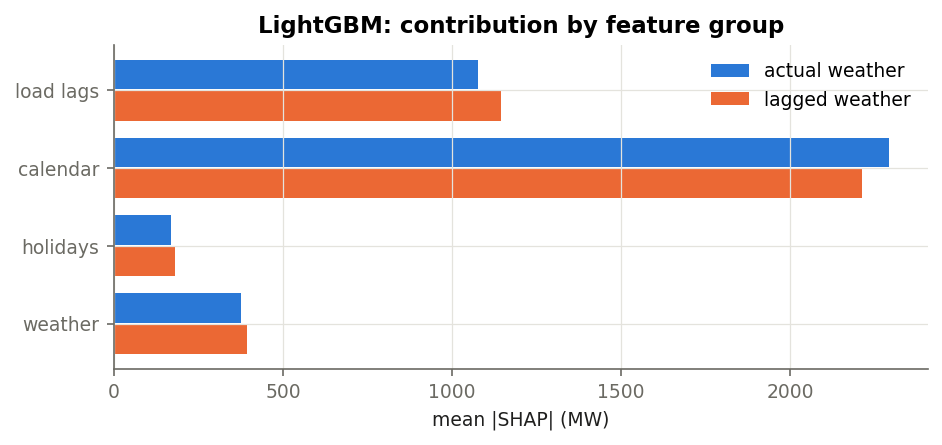
\includegraphics[width=\linewidth]{04_test_shap_groups.png}
    \caption{Mean $|\text{SHAP}|$ per feature group.}
  \end{subfigure}\hfill
  \begin{subfigure}[b]{0.56\linewidth}
    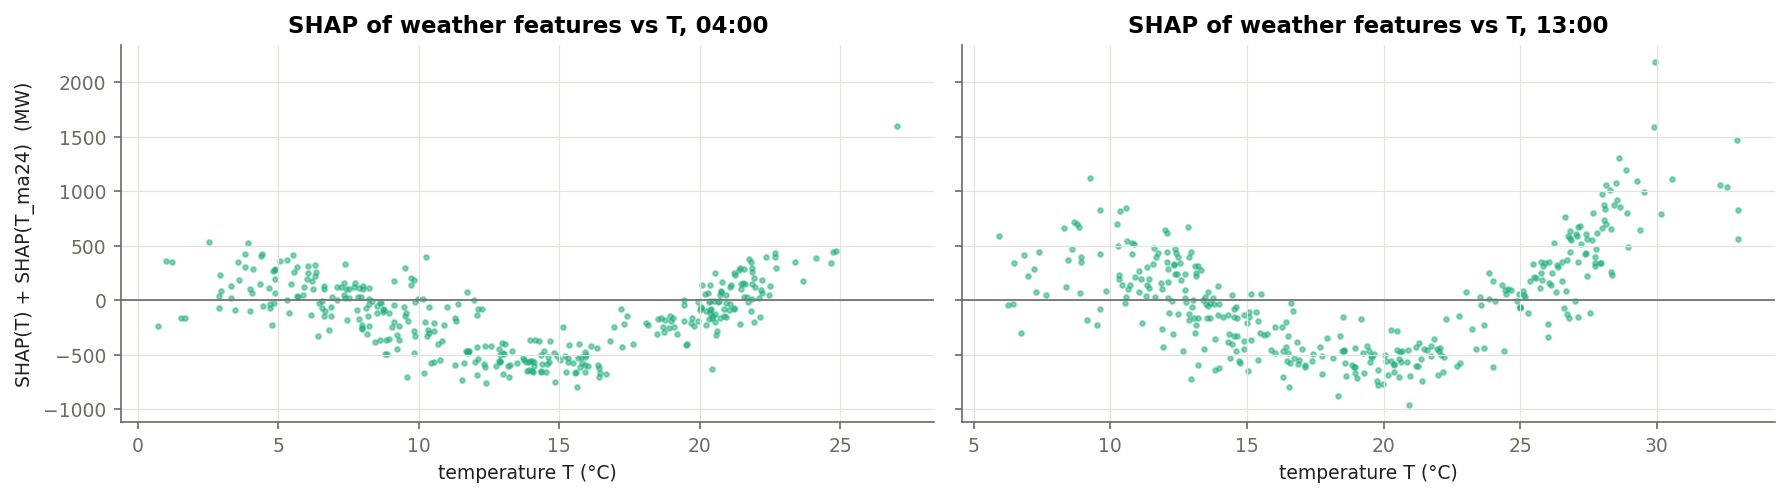
\includegraphics[width=\linewidth]{04_test_shap_temperature.png}
    \caption{Weather SHAP against temperature (actual).}
  \end{subfigure}
  \caption{SHAP explanation of LightGBM on the test year.}
  \label{fig:shap}
\end{figure}

\begin{itemize}
  \item \textbf{Calendar dominates} (mean $|$SHAP$|$ 2{,}292\,MW in the actual setting), mostly the
        hour of day (2{,}114\,MW) and weekday (698\,MW): the model first reproduces the daily and weekly
        shape. \textbf{Load lags} come second (1{,}077\,MW), then \textbf{weather} (375\,MW) and
        \textbf{holidays} (169\,MW). The lagged setting gives almost the same ranking, with more weight
        on $y_{D-7,h}$.
  \item \textbf{Weather} matters most in spring and late summer (482--554\,MW in April--May,
        512\,MW in August) and least in September and December (about 230--250\,MW).
  \item \textbf{Learned temperature response.} The weather SHAP has a clear U/V shape at both 04:00
        and 13:00, with its minimum around 15--20\,$^\circ$C and a steeper hot branch at midday
        (\cref{fig:shap}). This matches the V-shape with its kink at 18\,$^\circ$C that validation chose
        for Ridge, so the two models agree on the form of the response. Because temperature is
        correlated with season (\cref{tab:s2}), this shape describes what the model uses, not a causal
        effect of temperature.
\end{itemize}

\subsection{Comparison with the TSO Forecast}
\label{sec:eval-tso}

The TSO column has a test MAE of 268\,MW, about one sixth of our best model. It even follows the
unusual September days. This is consistent with the TSO using information we do not have (weather
forecasts, internal data, possibly updates after 10:00 on $D-1$). We report it only as context and
make no claim of beating or losing to it.
